%%%%%%%%%%%%%%%%%%%%%%%%%%%%%%%%%%%%%%%%%%%%%%%%%%%%%%%%%%%%%%%%%%%%%%%%%%%%%%%%
%  Policy Evaluation Lab -- Lecture 7: Instrumental variables and
%  regression discontinuity
%  Oct 2026 restructuring: both designs in one lecture, as designs rather
%  than estimators. IV part built from Overleaf "lecture 9.tex" (the PEL
%  version of the Migali IV deck): Angrist and Krueger, Wald estimator, LATE.
%  Dropped: North/South Carolina, Harmon and Walker, 2SLS tables.
%  RDD part is new (no RDD deck in the Migali material).
%  Sources checked for every number on the slides:
%   - Angrist and Krueger (1991), Wald table as reported in Angrist and Imbens
%     (1995): 5.892 / 5.905, 12.688 / 12.839, -0.0135 / -0.151 = 0.089; OLS
%     0.070; men born 1930-39, 1980 census (from the Migali deck).
%   - Lecture 5: 60% take-up, ITT 1.8, effect on investors 3 points.
%   - Bronzini and Iachini, Banca d'Italia version (2010 workshop): programme
%     of 2003, Regional Law 7/2002; scores 45/20/20/15, threshold 75 of 100;
%     sharp RDD; no overall effect; small firms raised investment by about
%     the grant, no effect for larger firms.
%   - de Blasio, Fantino and Pellegrini, Temi di discussione 792 (2011): RDD
%     on application date around an unexpected shortage of funds; applications
%     suspended after ten months, five years to reinstate funding; programme
%     not effective, public money substituted private.
%   - Cerqua and Pellegrini (2014), abstract on IDEAS/RePEc.
%%%%%%%%%%%%%%%%%%%%%%%%%%%%%%%%%%%%%%%%%%%%%%%%%%%%%%%%%%%%%%%%%%%%%%%%%%%%%%%%

\documentclass[aspectratio=169,xcolor=table]{beamer}
\input{preamble-pel}
\usetikzlibrary{positioning,arrows.meta,calc}
\newcolumntype{L}[1]{>{\raggedright\arraybackslash}p{#1}}

\title[Policy Evaluation Lab]{Policy Evaluation Lab}
\subtitle[Lecture 7]{Lecture 7: Instrumental variables and regression discontinuity}
\date[\pelYear]{October, 2026}

\begin{document}

\frame{\titlepage}

\begin{frame}{Where we are}
\small
\bi
  \item Monday: difference-in-differences, a comparison group followed over time
  \item Today: two designs that exploit \textbf{rules}
    \bi
      \item \textbf{Instrumental variables}: something outside the firm's control pushes some units into treatment
      \item \textbf{Regression discontinuity}: a cut-off decides who is treated
    \ei
\ei
\vspace{0.1cm}
\centering\footnotesize
\begin{tabular}{L{3.6cm}L{5.0cm}L{4.8cm}}
\toprule
\textbf{Design} & \textbf{The comparison group} & \textbf{Key assumption} \\
\midrule
Instrumental variables & units the outside factor did not push & the factor works only through the treatment \\
Regression discontinuity & units just below the cut-off & no sorting around the cut-off \\
\bottomrule
\end{tabular}
\end{frame}

%%%%%%%%%%%%%%%%%%%%%%%%%%%%%%%%%%%%%%%%%%%%%%%%%%%%%%%%%%%%%%%%%%%%%%%%%%%%%%%%
\section{Instrumental variables}

\begin{frame}{You have already used an instrument}
\small
Lecture 5, our grant lottery:
\bi
  \item Winning the lottery is \textbf{random}, but only 60\% of winners actually invest
  \item Comparing winners and losers gives the effect of the \textbf{offer}: ITT $=$ 1.8 points
  \item The effect on firms that \textbf{invest} because they won:
\ei
\[ \frac{\text{effect of winning on sales growth}}{\text{effect of winning on investing}} = \frac{1.8}{0.60} = 3 \text{ points} \]
\begin{block}{}
The lottery is an \textbf{instrument}: it changes who gets treated, at random, and has no other way to affect the outcome
\end{block}
\pelTableNote{Instrumental variables generalise this ratio to situations where nobody ran a lottery, but something else played its role.}
\end{frame}

\begin{frame}{The idea}
\centering
\begin{tikzpicture}[node distance=2.6cm, every node/.style={font=\small},
    box/.style={draw=pelBorder, fill=pelBgAlt, rounded corners=3pt, minimum width=2.6cm, minimum height=0.9cm, align=center}]
  \node[box, draw=pelAccent, fill=pelAccentLight] (z) {\textbf{Instrument} $Z$\\ e.g.\ the lottery};
  \node[box, right=of z] (d) {\textbf{Treatment} $D$\\ investing};
  \node[box, right=of d] (y) {\textbf{Outcome} $Y$\\ sales growth};
  \node[box, above=0.8cm of $(d)!0.5!(y)$] (u) {unobserved: motivation, management};
  \draw[-{Stealth}, pelAccent, line width=1.1pt] (z) -- node[above, font=\scriptsize]{1. relevance} (d);
  \draw[-{Stealth}, line width=1.1pt] (d) -- (y);
  \draw[-{Stealth}, pelMuted] (u) -- (d);
  \draw[-{Stealth}, pelMuted] (u) -- (y);
  \draw[-{Stealth}, pelDanger, dashed, line width=0.9pt] (z.south) to[bend right=25] node[below, font=\scriptsize]{2. exclusion: no direct path} (y.south);
\end{tikzpicture}

\raggedright\small
\be
  \item \textbf{Relevance}: $Z$ clearly changes the treatment (checkable in the data)
  \item \textbf{Exclusion}: $Z$ affects the outcome \textbf{only} through the treatment (not checkable: an argument)
  \item $Z$ is as good as random: unrelated to motivation, ability, management
\ee
\end{frame}

\begin{frame}{The Wald ratio}
\begin{block}{Effect of the treatment}
\[ \rho = \frac{\text{difference in outcomes between } Z=1 \text{ and } Z=0}{\text{difference in treatment between } Z=1 \text{ and } Z=0} = \frac{\text{reduced form}}{\text{first stage}} \]
\end{block}
\small
\bi
  \item \textbf{First stage}: how much the instrument moves the treatment. If it barely moves it (a \textbf{weak} instrument), we divide by almost zero and the estimate is unreliable
  \item \textbf{Reduced form}: how much the instrument moves the outcome
  \item With controls and several instruments, software runs ``two-stage least squares'': same logic, same ratio
\ei
\end{frame}

\begin{frame}{A classic: quarter of birth and schooling (Angrist and Krueger, 1991)}
\small
\bi
  \item Question: what is the return to one more year of school? Comparing educated and less educated people mixes school with ability and family background
  \item In the US, children start school in the calendar year they turn 6, and may leave at 16
  \item Those born early in the year reach 16 after fewer years of school: if they leave as soon as allowed, they have \textbf{slightly less schooling}
  \item The month of birth is unrelated to ability or family: a natural instrument
\ei
\end{frame}

\begin{frame}{Quarter of birth: first stage and reduced form}
\begin{columns}[T]
\begin{column}{0.48\textwidth}
\centering
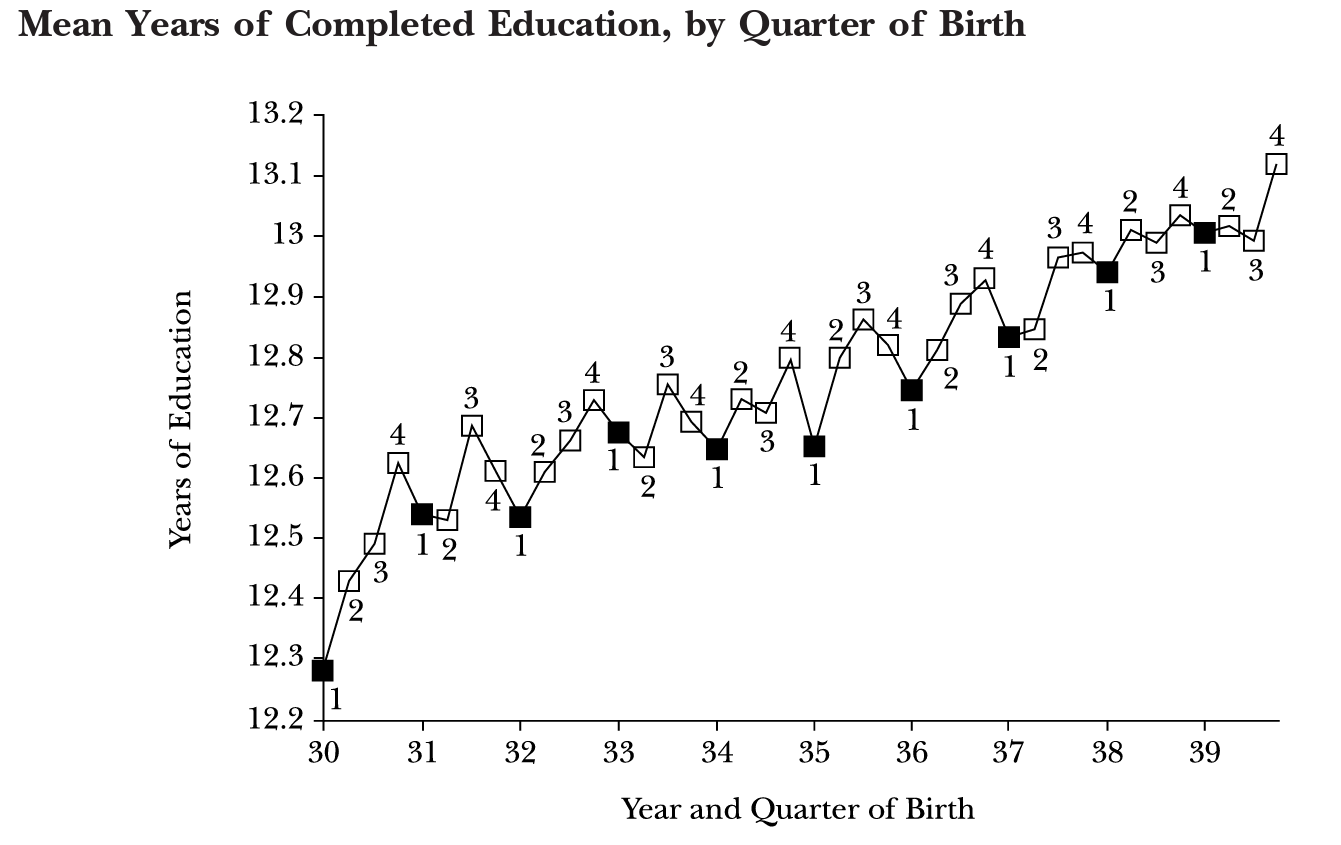
\includegraphics[width=\linewidth]{figures/lecture-07ivrd/fig_qob-educ.jpeg}
\pelTableNote{First stage: schooling by quarter of birth.}
\end{column}
\begin{column}{0.48\textwidth}
\centering
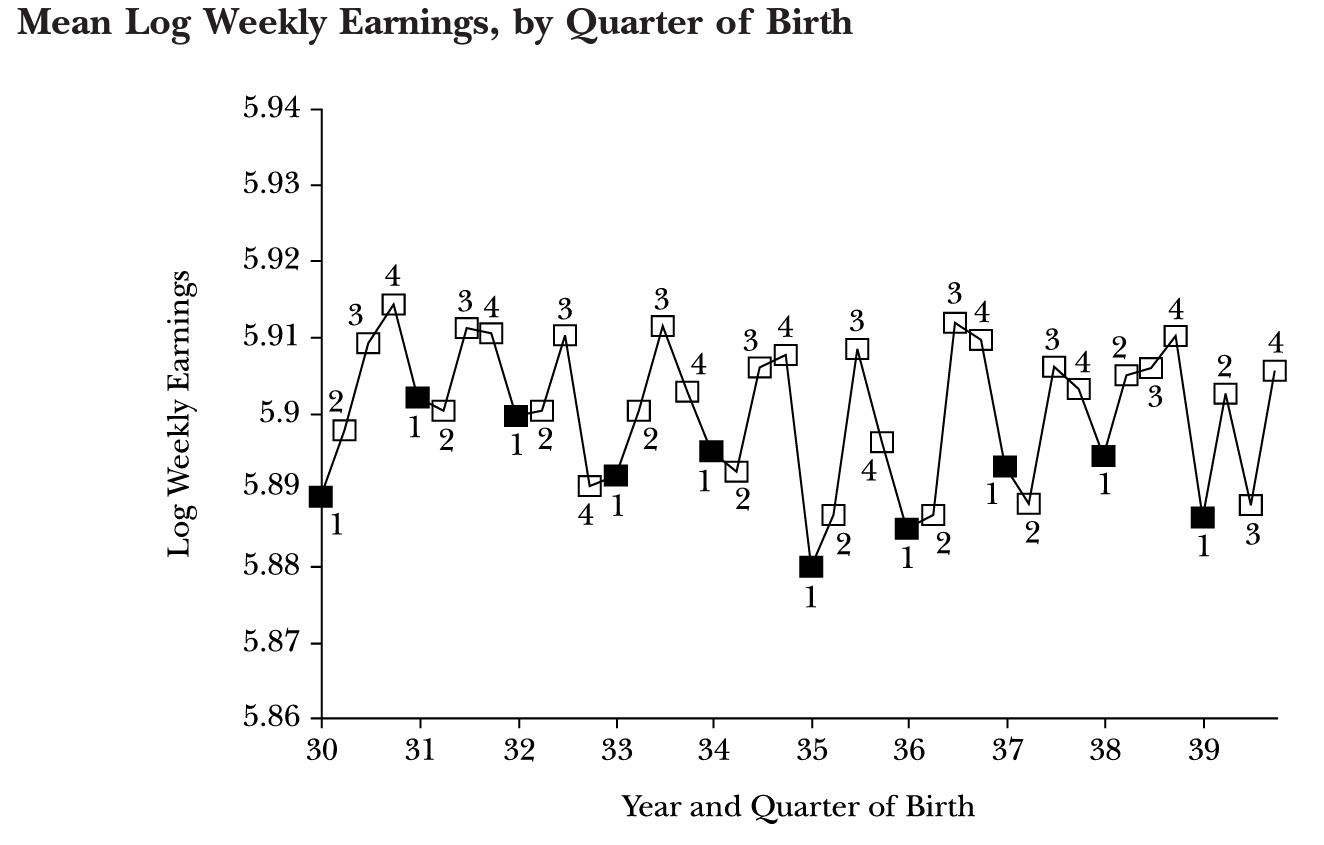
\includegraphics[width=\linewidth]{figures/lecture-07ivrd/fig_qob-earn.jpeg}
\pelTableNote{Reduced form: earnings by quarter of birth.}
\end{column}
\end{columns}
\vspace{0.1cm}
\small Men born early in the year have slightly less schooling \textbf{and} slightly lower earnings: if the only link is schooling, the ratio of the two gaps is the return to school
\end{frame}

\begin{frame}{The result}
\begin{columns}[T]
\begin{column}{0.58\textwidth}
\centering\footnotesize
\begin{tabular}{lrrr}
\toprule
 & \textbf{Born Q1} & \textbf{Born Q4} & \textbf{Difference} \\
\midrule
log weekly wage & 5.892 & 5.905 & $-0.0135$ \\
years of school & 12.688 & 12.839 & $-0.151$ \\
\midrule
\multicolumn{3}{l}{\textbf{Wald estimate}: $-0.0135 / -0.151$} & \textbf{0.089} \\
\multicolumn{3}{l}{OLS (simple comparison)} & 0.070 \\
\bottomrule
\end{tabular}
\pelTableNote{Men born 1930--39, 1980 US census. Angrist and Krueger (1991), as reported in Angrist and Imbens (1995).}
\end{column}
\begin{column}{0.38\textwidth}
\small
\bi
  \item One more year of school raises earnings by about \textbf{9\%}
  \item The whole estimate rests on a tiny difference: 0.15 years of school
  \item Exclusion: could the month of birth affect earnings in other ways? (age at school entry, season of birth and health)
\ei
\end{column}
\end{columns}
\end{frame}

\begin{frame}{Whose effect? Compliers}
\small
An instrument moves only some units. Four types:
\bi
  \item \textbf{Always-takers}: treated anyway (e.g.\ would invest even without the grant)
  \item \textbf{Never-takers}: never treated (would not invest even with it)
  \item \textbf{Compliers}: treated \textbf{because of} the instrument
  \item Defiers: do the opposite (assumed away)
\ei
\begin{block}{Local average treatment effect (LATE)}
IV measures the effect for the \textbf{compliers} only. Angrist and Krueger: men who stayed in school because the law kept them there. Our lottery: firms that invested because they won
\end{block}
\pelTableNote{For policy this is often the relevant group: the firms that a policy actually moves.}
\end{frame}

\begin{frame}{Instruments in business and policy}
\small
\bi
  \item \textbf{Encouragement}: a programme open to all; some firms get a randomly assigned call or visit, the instrument for taking part
  \item \textbf{Rules}: assignment by date or by a randomly assigned official
  \item \textbf{Distance} to a bank or university, for credit or education: exclusion often doubtful
\ei
\begin{alertblock}{Where IV goes wrong}
\bi
  \item \textbf{Weak first stage}: the instrument hardly moves the treatment
  \item \textbf{Exclusion fails}: the instrument has its own path to the outcome. Not testable: it must be argued
\ei
\end{alertblock}
\end{frame}

%%%%%%%%%%%%%%%%%%%%%%%%%%%%%%%%%%%%%%%%%%%%%%%%%%%%%%%%%%%%%%%%%%%%%%%%%%%%%%%%
\section{Regression discontinuity}

\begin{frame}{Rules with a cut-off}
\small
\bi
  \item Many policies assign treatment by a \textbf{score} and a \textbf{threshold}:
    \bi
      \item a grant to projects scoring 75 or more
      \item a tax rule for firms below 50 employees
      \item a subsidy for municipalities under 5,000 inhabitants
    \ei
  \item Firms far above and far below the threshold differ a lot
  \item Firms at 74 and at 76 are almost identical, except that one is funded
\ei
\begin{block}{The idea}
Compare units \textbf{just above} and \textbf{just below} the cut-off: near the threshold, treatment is as good as random
\end{block}
\end{frame}

\begin{frame}{The picture}
\centering
\begin{tikzpicture}
\begin{axis}[pel chart, width=0.8\textwidth, height=0.66\textheight,
    xmin=50, xmax=100, ymin=0, ymax=14, xtick={60,75,90}, ytick=\empty,
    xlabel={project score}, ylabel={investment after the call}, clip=false]
  \addplot[only marks, mark=*, mark size=1.2pt, pelSlate!70, samples=26, domain=51:74.5] {2+0.08*(x-50)+1.2*sin(deg(7*x))};
  \addplot[only marks, mark=*, mark size=1.2pt, pelAccent!70, samples=26, domain=75.5:99] {6+0.08*(x-50)+1.2*sin(deg(7*x))};
  \addplot[pelSlate, line width=1.3pt, domain=50:75] {2+0.08*(x-50)};
  \addplot[pelAccent, line width=1.3pt, domain=75:100] {6+0.08*(x-50)};
  \draw[pelText, dashed] (axis cs:75,0) -- (axis cs:75,13.5);
  \node[font=\scriptsize, anchor=south] at (axis cs:75,13.5) {cut-off};
  \draw[pelText, <->, line width=0.8pt] (axis cs:76.5,4) -- (axis cs:76.5,8);
  \node[font=\footnotesize, anchor=west] at (axis cs:77,6) {effect at the cut-off};
  \node[font=\scriptsize, text=pelSlate] at (axis cs:58,1) {not funded};
  \node[font=\scriptsize, text=pelAccent] at (axis cs:93,12.6) {funded};
\end{axis}
\end{tikzpicture}
\pelTableNote{Illustrative data. Without the grant, the two lines would join smoothly at 75; the jump is the effect.}
\end{frame}

\begin{frame}{What must hold, and how to check it}
\small
\begin{block}{The assumption}
Nothing else jumps at the cut-off, and units cannot \textbf{precisely} place themselves on one side
\end{block}
\bi
  \item \textbf{Sorting}: firms able to push their score just above the line differ from those just below. Check: suspiciously many units just above?
  \item \textbf{Balance}: size, sector, age (fixed before the call) should not jump at the cut-off
  \item \textbf{Other rules at the same threshold}: if 50 employees triggers other obligations too, the jump mixes them
\ei
\pelTableNote{The price: the effect is \textbf{local}. A grant that works for projects scoring 75 may not work for those scoring 95.}
\end{frame}

\begin{frame}{R\&D grants in Emilia-Romagna (Bronzini and Iachini, 2014)}
\small
\bi
  \item 2003: the Region funds industrial research and pre-competitive development; an independent committee scores each project:
\ei
\centering\footnotesize
\begin{tabular}{lr}
\toprule
technical and scientific & up to 45 points \\
financial and economic & up to 20 points \\
managerial & up to 20 points \\
regional impact & up to 15 points \\
\midrule
\textbf{funded if total $\geq$ 75} (out of 100) & \\
\bottomrule
\end{tabular}
\vspace{0.1cm}

\raggedright\small
\bi
  \item A \textbf{sharp} RDD: compare investment of firms just above and just below 75
  \item Firms could hardly control their score. But there are \textbf{fewer} projects at 74 than expected: the authors' reading is that the committee avoided scoring a project just below the line
\ei
\end{frame}

\begin{frame}{What they found}
\small
\bi
  \item All firms together: \textbf{no significant increase} in investment. Firms partly replaced their own money with public money (crowding out)
  \item By size:
    \bi
      \item \textbf{small} firms increased investment by about the amount of the grant
      \item \textbf{larger} firms: no additional investment
    \ei
\ei
\begin{exampleblock}{The policy lesson}
The same euro has different effects on different firms. A result like this argues for \textbf{targeting} the grants on small firms, which are more likely to be short of finance
\end{exampleblock}
\pelTableNote{Remember Lecture 5: a ``no effect'' on the whole sample can hide a real effect on a subgroup, and vice versa.}
\end{frame}

\begin{frame}{A cut-off in time: an unexpected shortage of funds}
\small
\begin{columns}[T]
\begin{column}{0.55\textwidth}
\bi
  \item de Blasio, Fantino and Pellegrini (2011): a national fund for technological innovation
  \item At some point the money ran out, unexpectedly. Firms could still apply, hoping funds would return
  \item Applications were suspended after ten months; funding took five years to come back
  \item Comparison: firms that applied \textbf{just before} the shortage (funded) and \textbf{just after} (not funded)
\ei
\end{column}
\begin{column}{0.42\textwidth}
\begin{block}{Result}
The programme did not raise innovative investment: public funding replaced private funding
\end{block}
\pelTableNote{The cut-off is the date of application, not a score. The key question: did the firms that applied after the shortage differ from those that applied before?}
\end{column}
\end{columns}
\end{frame}

\begin{frame}{Law 488 again: many cut-offs}
\small
\bi
  \item Law 488 ranked applicants by region and call, and funded them until the money ran out: \textbf{each ranking has its own cut-off}
  \item Cerqua and Pellegrini (2014) compare firms just above and just below each cut-off
  \item They find positive effects on investment, employment and turnover, \textbf{not} due to investment brought forward
\ei
\vspace{0.1cm}
\begin{alertblock}{Two designs, two answers}
Monday, Bronzini and de Blasio (DiD, all funded vs all rejected): part of the investment was only brought forward. Today, Cerqua and Pellegrini (RDD, near the cut-offs): real additional investment. Different samples, periods and methods: which one would you show a minister, and why?
\end{alertblock}
\end{frame}

\begin{frame}{Sharp and fuzzy: where the two designs meet}
\small
\bi
  \item \textbf{Sharp} RDD: crossing the cut-off decides treatment for everyone (Emilia-Romagna)
  \item \textbf{Fuzzy} RDD: crossing the cut-off only raises the \textbf{probability} of treatment (some funded firms renounce, some below get money elsewhere)
\ei
\begin{block}{}
In a fuzzy RDD, being above the cut-off is an \textbf{instrument}: effect $=$ jump in the outcome $/$ jump in the probability of treatment. The same ratio as the lottery and as quarter of birth
\end{block}
\end{frame}

%%%%%%%%%%%%%%%%%%%%%%%%%%%%%%%%%%%%%%%%%%%%%%%%%%%%%%%%%%%%%%%%%%%%%%%%%%%%%%%%
\section{Reading IV and RDD studies}

\begin{frame}{Questions to ask}
\small
\begin{columns}[T]
\begin{column}{0.48\textwidth}
\textbf{Instrumental variables}
\be
  \item Does the instrument clearly move the treatment?
  \item Can you think of any other path from the instrument to the outcome?
  \item Who are the compliers, and do we care about them?
\ee
\end{column}
\begin{column}{0.48\textwidth}
\textbf{Regression discontinuity}
\be
  \item Who sets the score, and could units manipulate it?
  \item Does anything else change at the cut-off?
  \item Is the effect near the cut-off the one the policy question needs?
\ee
\end{column}
\end{columns}
\vspace{0.2cm}
\begin{block}{}
\centering Both designs buy credibility with \textbf{locality}: a convincing effect for a specific group, not for everyone
\end{block}
\end{frame}

\begin{frame}{Next}
\small
\bi
  \item \textbf{Friday}: lab and discussion
  \item \textbf{Next week}: synthetic control, and reading an evaluation critically. End of Part I
  \item Readings on the Lectures page, week 4
\ei
\end{frame}

\begin{frame}{References}
\tiny
\bi
  \item Angrist, J. D. and G. W. Imbens (1995), Two-stage least squares estimation of average causal effects in models with variable treatment intensity, \textit{Journal of the American Statistical Association}, 90(430), 431--442
  \item Angrist, J. D. and A. B. Krueger (1991), Does compulsory school attendance affect schooling and earnings?, \textit{Quarterly Journal of Economics}, 106(4), 979--1014
  \item Bronzini, R. and E. Iachini (2014), Are incentives for R\&D effective? Evidence from a regression discontinuity approach, \textit{American Economic Journal: Economic Policy}, 6(4), 100--134
  \item Bronzini, R. and G. de Blasio (2006), Evaluating the impact of investment incentives: the case of Italy's Law 488/1992, \textit{Journal of Urban Economics}, 60(2), 327--349
  \item Cerqua, A. and G. Pellegrini (2014), Do subsidies to private capital boost firms' growth? A multiple regression discontinuity design approach, \textit{Journal of Public Economics}, 109, 114--126
  \item de Blasio, G., D. Fantino and G. Pellegrini (2011), Evaluating the impact of innovation incentives: evidence from an unexpected shortage of funds, Banca d'Italia, Temi di discussione 792
\ei
\end{frame}

\pelQuestions

\end{document}
